\documentclass[main.tex]{subfiles}

\begin{document}
\chapter{Exploration of Composition Profiles for Chapter~\ref{ch:tn_v_ec_sn} Models}\label{apx:composition}
In the pursuit of a comprehensive understanding of stellar evolution, this thesis delves into the intricate details of various stellar models, exploring the nuances of their composition profiles. While the main body of the thesis provides a thorough examination of key findings and essential discussions, the complexity and richness of the data necessitate the inclusion of supplementary material. This supplementary information, presented in Appendix A, serves to enhance the depth of our analysis by offering a more extensive look at the composition profiles for a diverse array of stellar models.

The decision to include this appendix stems from the recognition that certain detailed figures depicting composition profiles may not seamlessly integrate into the narrative flow of the primary chapters. In order to maintain clarity and coherence in the main text, these additional figures have found a home in this dedicated appendix. These figures offer a visual supplement to the theoretical discussions within the main chapters, providing a comprehensive overview of the intricate interplay between different stellar parameters and their corresponding composition profiles.
% \clearpage

\section{The \seriesone Grid}

\begin{figure*}[hbt!]
    \centering
    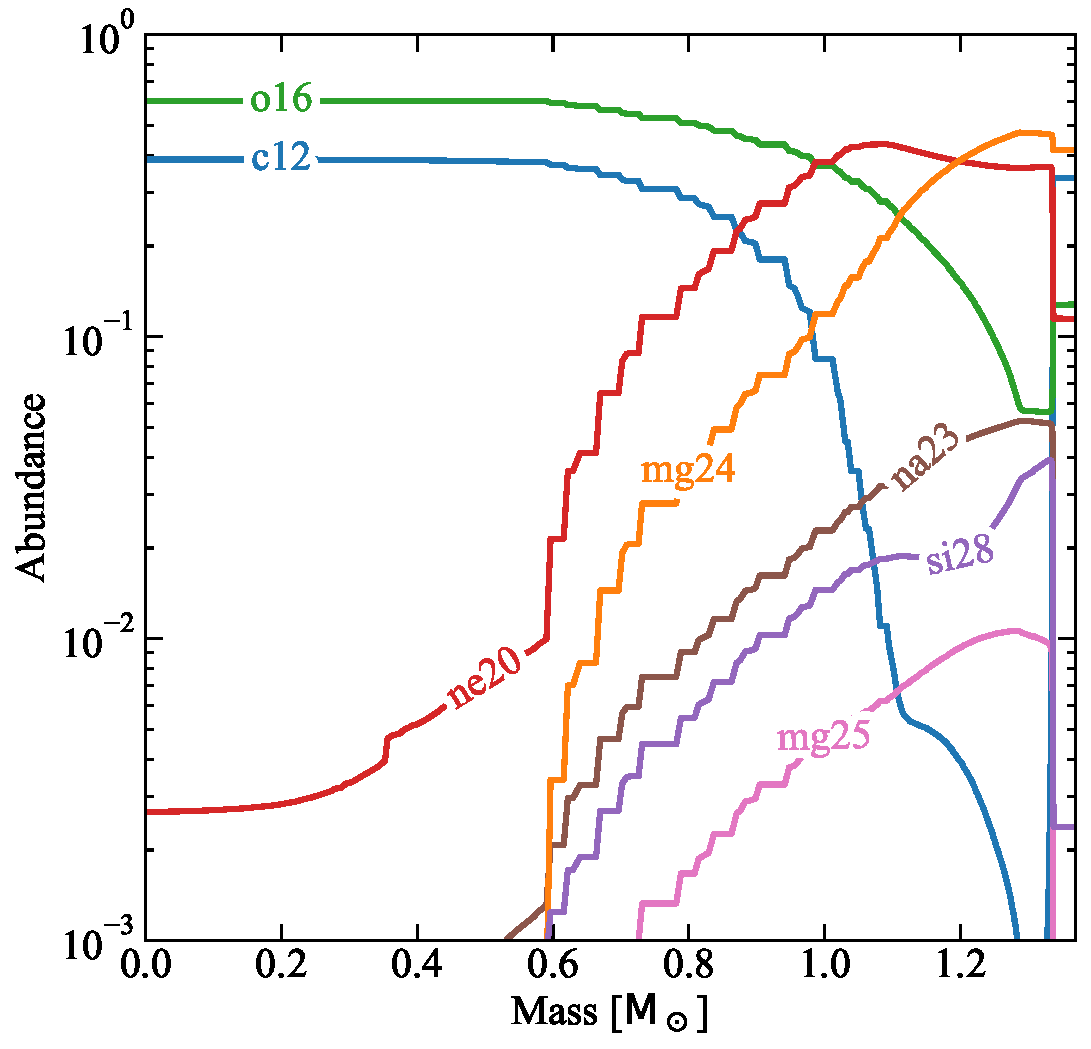
\includegraphics[height=8cm]{figures/chapter2/abundances/1p8_logRho9_abun.pdf}\quad
    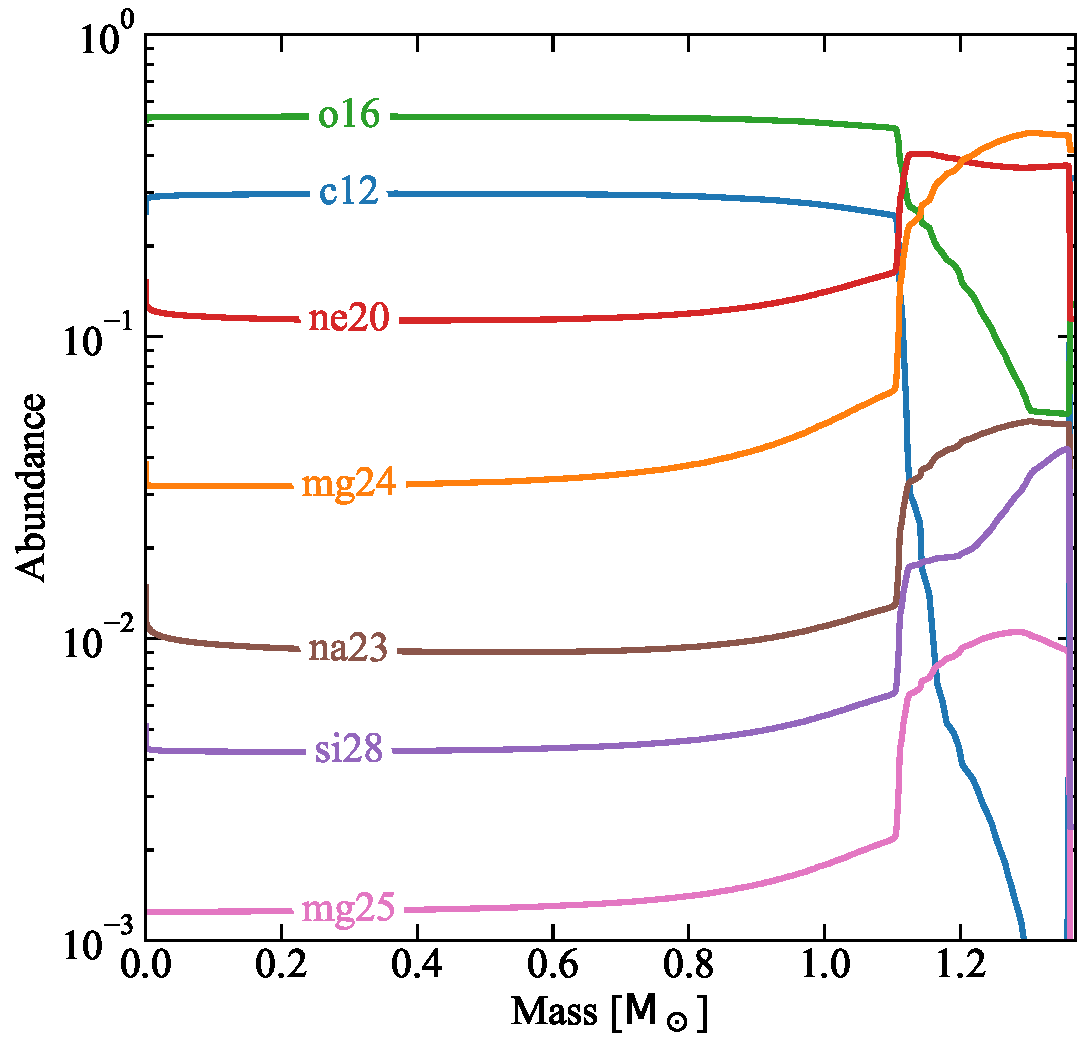
\includegraphics[height=8cm]{figures/chapter2/abundances/1p8_final_abun.pdf}
    \caption{Abundance profiles of the \seriesone hybrid stellar model with $ 1.8\msun,  Z=0.02;f_{OV}=0.014$. The left panel refers to the structure when $\rm \log(\rho_c / g \ cm^{-3}) \simeq 9.0$ (indicated by the black cross-mark in Fig.~\ref{fig:RhoT}). The right panel shows the final chemical composition of the model.} 
\end{figure*}

\begin{figure*}[hbt!]
    \centering
    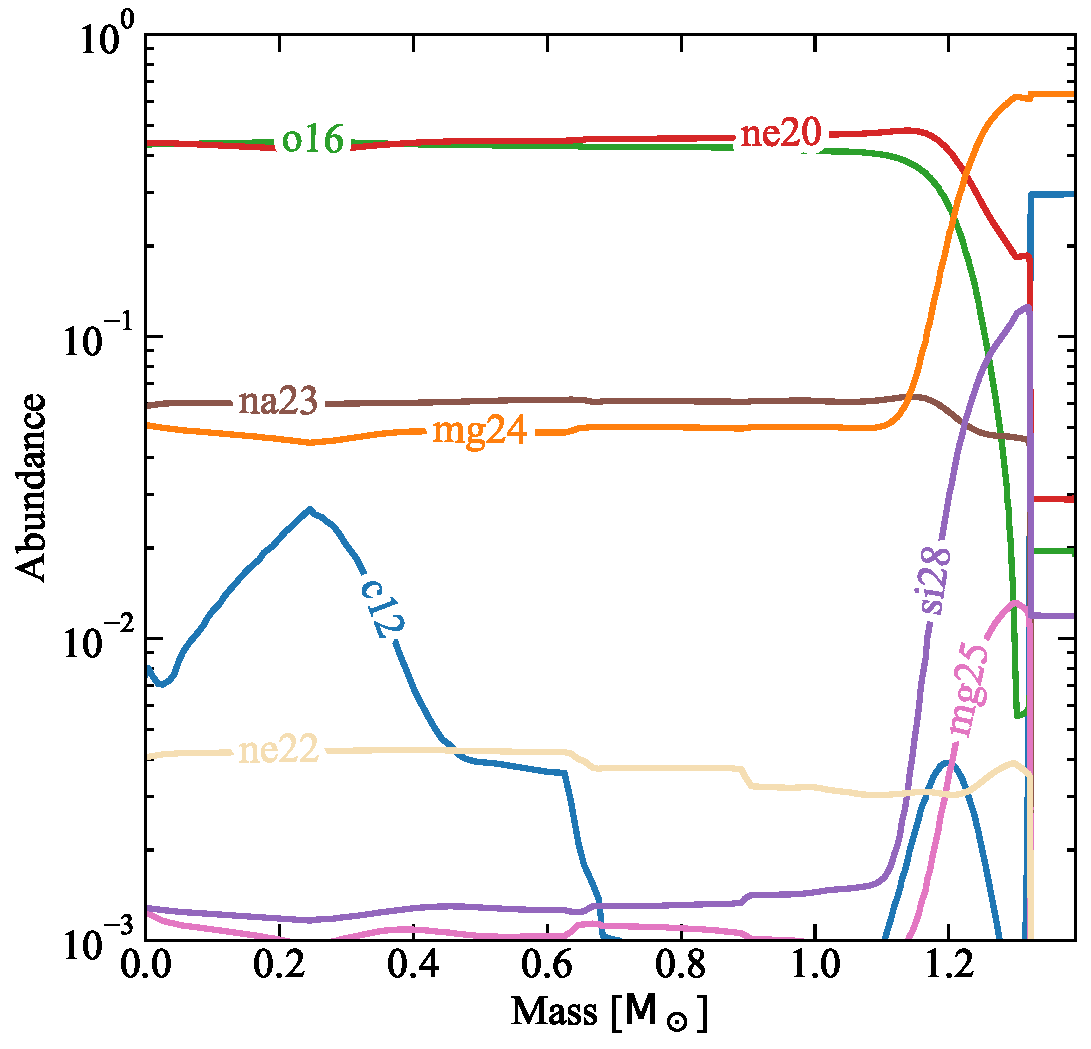
\includegraphics[height=8cm]{figures/chapter2/abundances/2p5_logRho_9_abun.pdf}\quad
    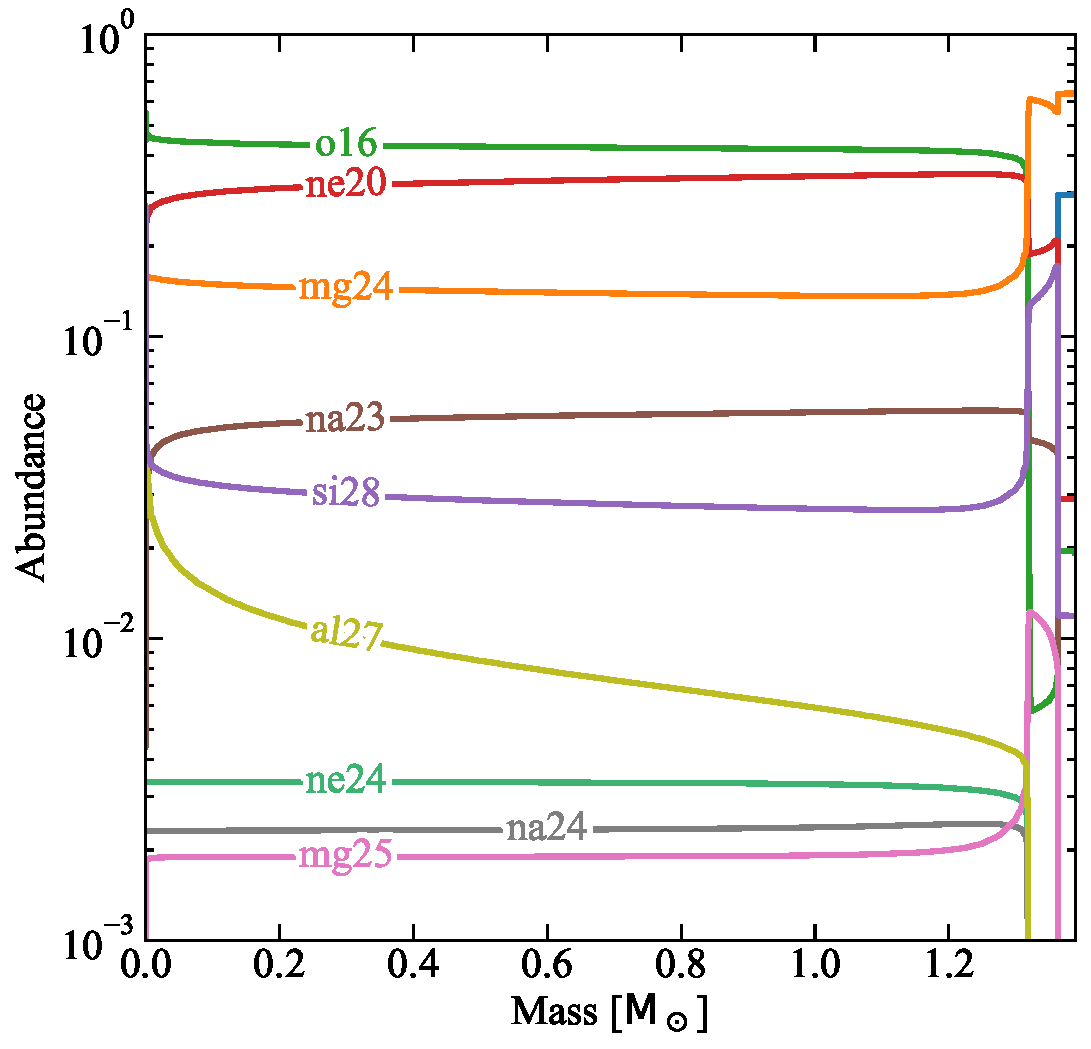
\includegraphics[height=8cm]{figures/chapter2/abundances/2p5_final_abun.pdf}\par\medskip
    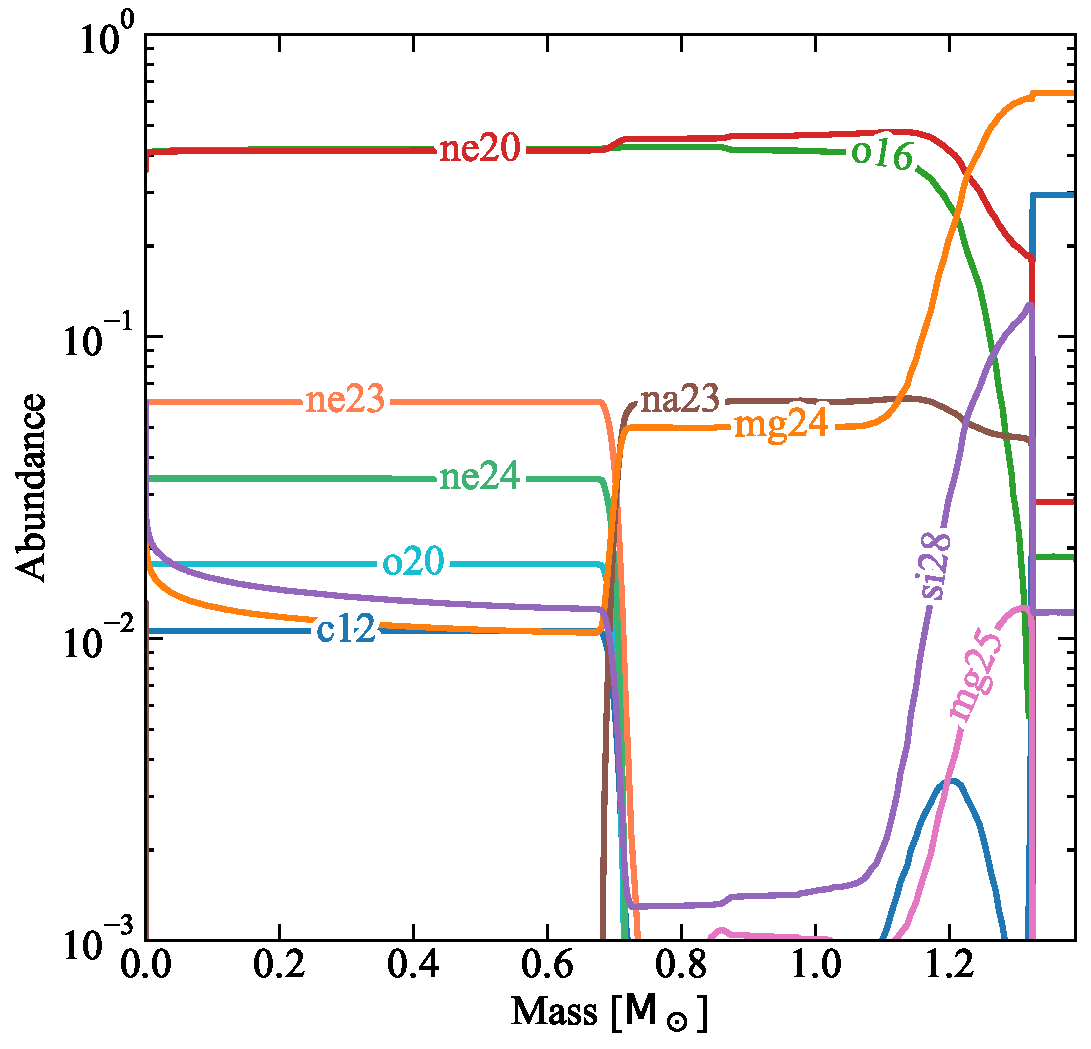
\includegraphics[height=8cm]{figures/chapter2/abundances/2p5_abun_carbon_sup.pdf}
    \caption{Abundance profiles of the \seriesone $ 2.5\msun,  Z=0.02;f_{OV}=0.0$ stellar model. The top-left panel refers to the structure when $\rm \log(\rho_c / g \ cm^{-3}) \simeq 9.0$. The distribution of residual carbon from previous burning stages is visible. The top-right panel shows the final composition of this model. Ignition of residual carbon leads to thermonuclear explosion.
    The panel at the bottom shows the final structure of the same model, in the case where carbon-consuming nuclear reactions have been turned off.
    In this scenario, the core reaches the density threshold for $e$-captures on Ne nuclei to commence, leading to formation of \iso{O}{20}, and most likely to an ECSN.}
    \label{apx:fig:eta1p0}
\end{figure*}


\clearpage
\section{The \seriestwo Grid}

\begin{figure*}[hbt!]
    \centering 
    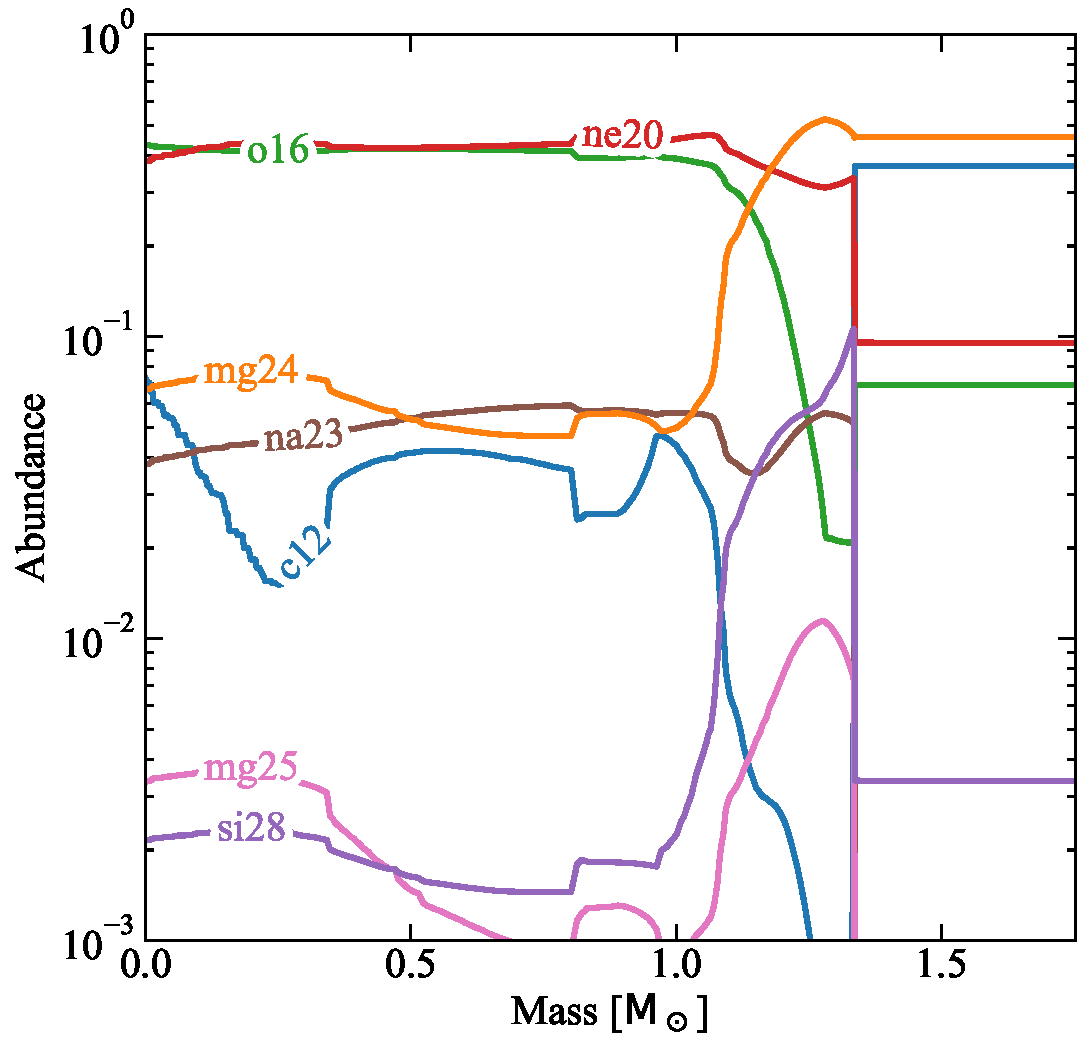
\includegraphics[height=8cm]{figures/chapter2/abundances/2p0_eta0p25_Rho9.pdf}\quad
    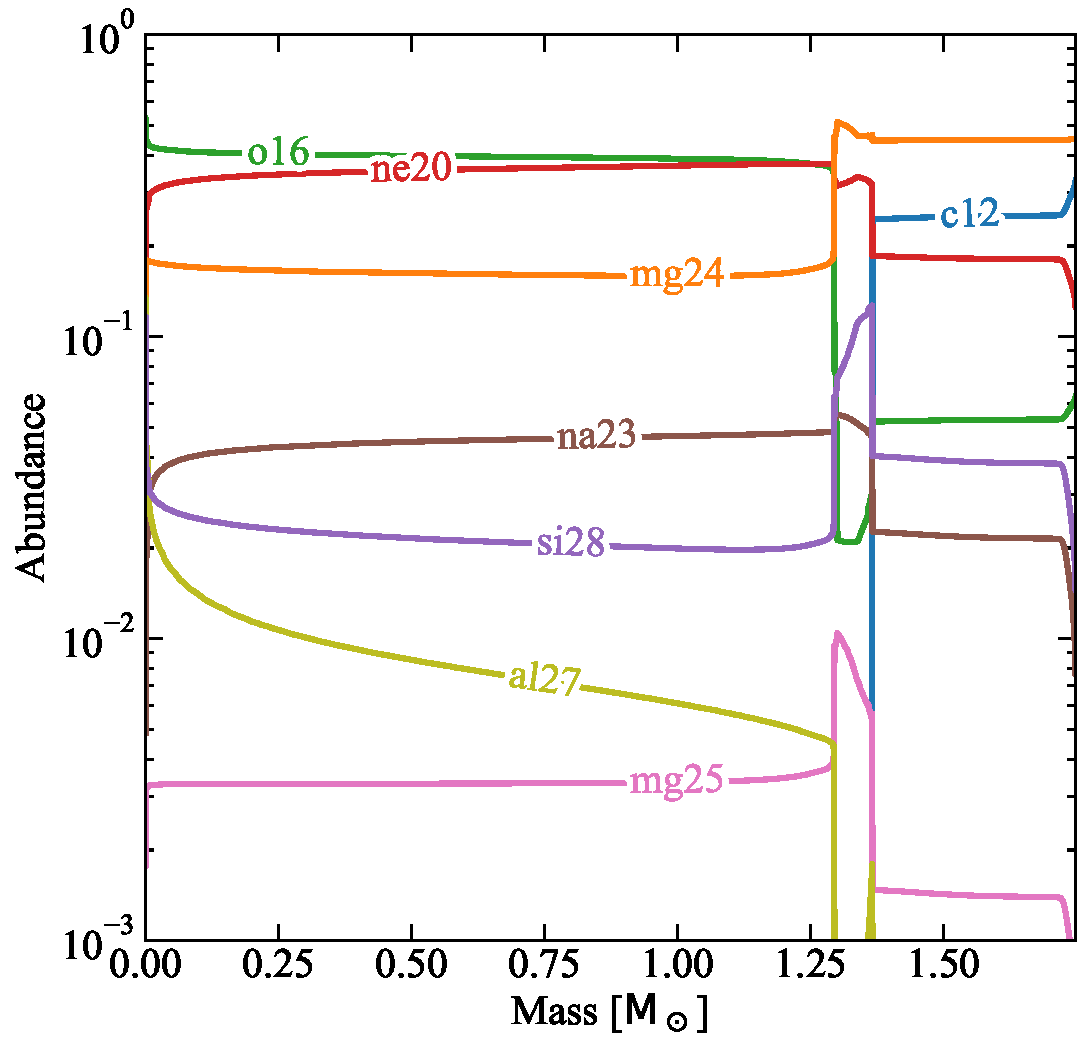
\includegraphics[height=8cm]{figures/chapter2/abundances/2p0_eta0p25_final_abun.pdf}
    \caption{Abundance profiles of the \seriestwo $ 2.0\msun,  Z=0.02;f_{OV}=0.0; \eta=0.25$ stellar model. The left panel refers to the structure when $\rm \log(\rho_c / g \ cm^{-3}) \simeq 9.0$ (shortly before the Urca cooling phase). The right panel shows the final chemical composition of the model after the ignition of neon.}
    \label{apx:fig:eta0p25}
\end{figure*}

\begin{figure*}[hbt!]
    \centering 
    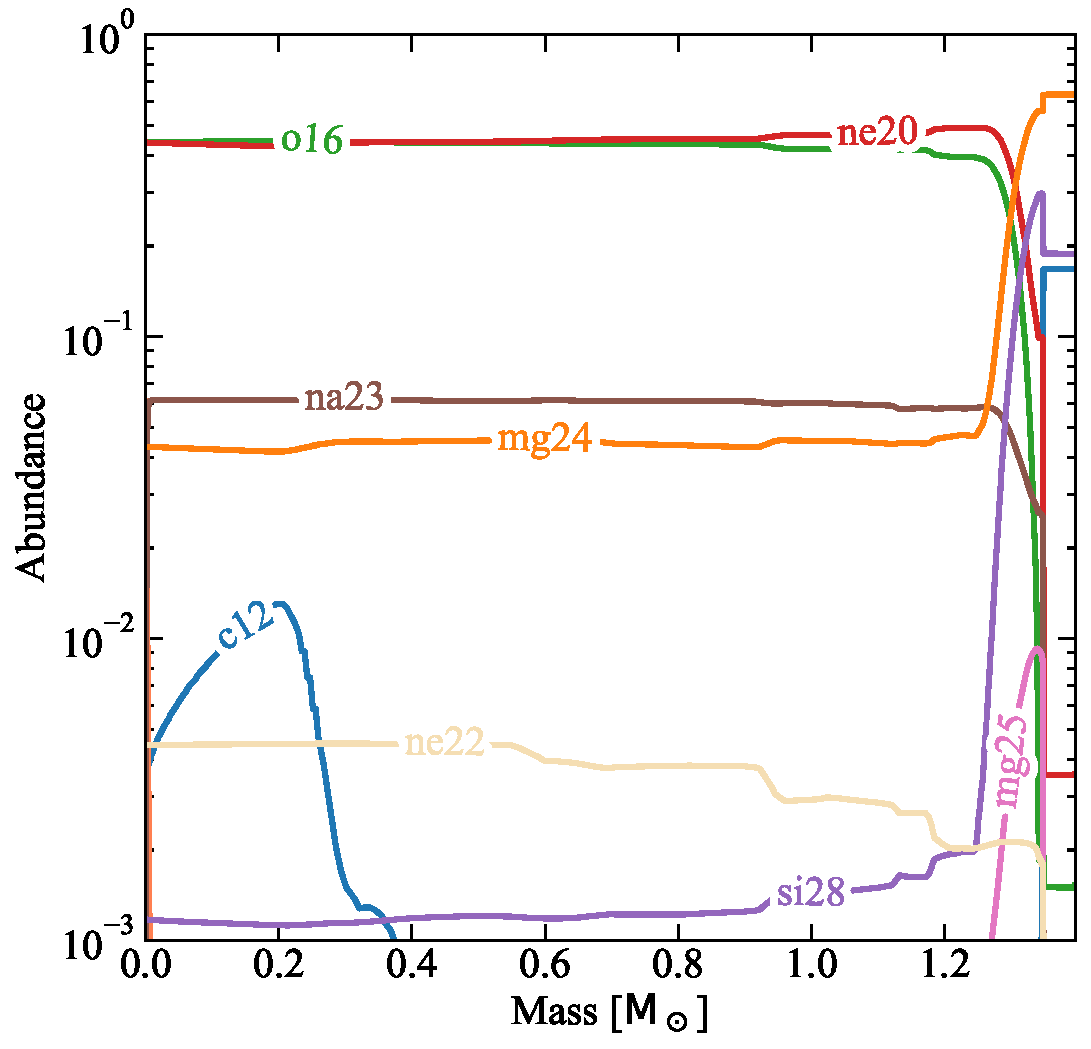
\includegraphics[height=8cm]{figures/chapter2/abundances/2p7_eta0p8_Rho9.pdf}\quad
    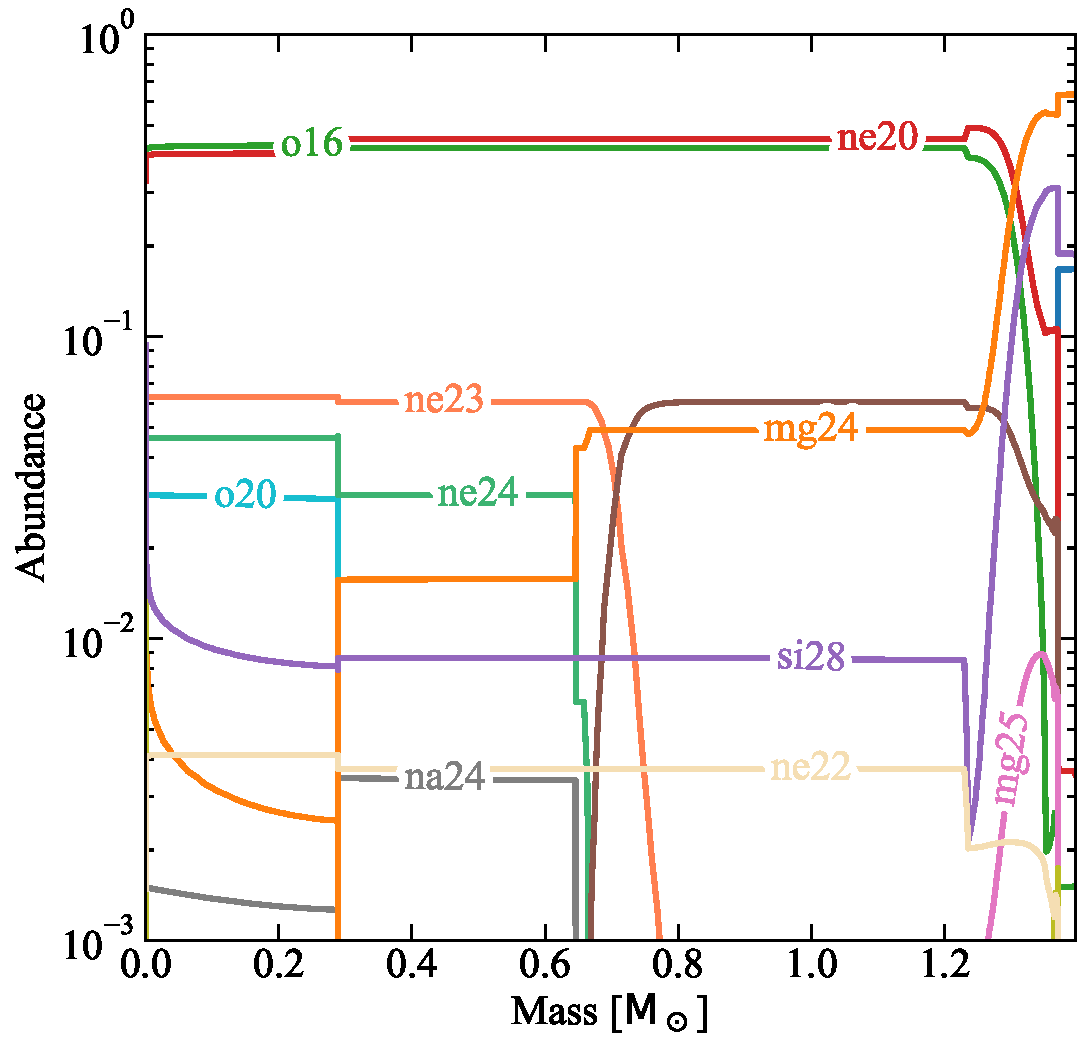
\includegraphics[height=8cm]{figures/chapter2/abundances/2p7_eta0p8_final_abun.pdf}
    \caption{Abundance profiles of the \seriestwo $ 2.7\msun,  Z=0.02;f_{OV}=0.0; \eta=0.8$ stellar model. The left panel refers to the structure when $\rm \log(\rho_c / g \ cm^{-3}) \simeq 9.0$ (shortly before the Urca cooling phase). The right panel shows the final chemical composition of the model after the ignition of neon. This model has reached the critical density for $e$-captures on \iso{Ne}{20} which leads to the formation of \iso{O}{20} (cyan line).}
    \label{apx:fig:eta0p8}
\end{figure*}

\begin{figure*}[hbt!]
    \centering 
    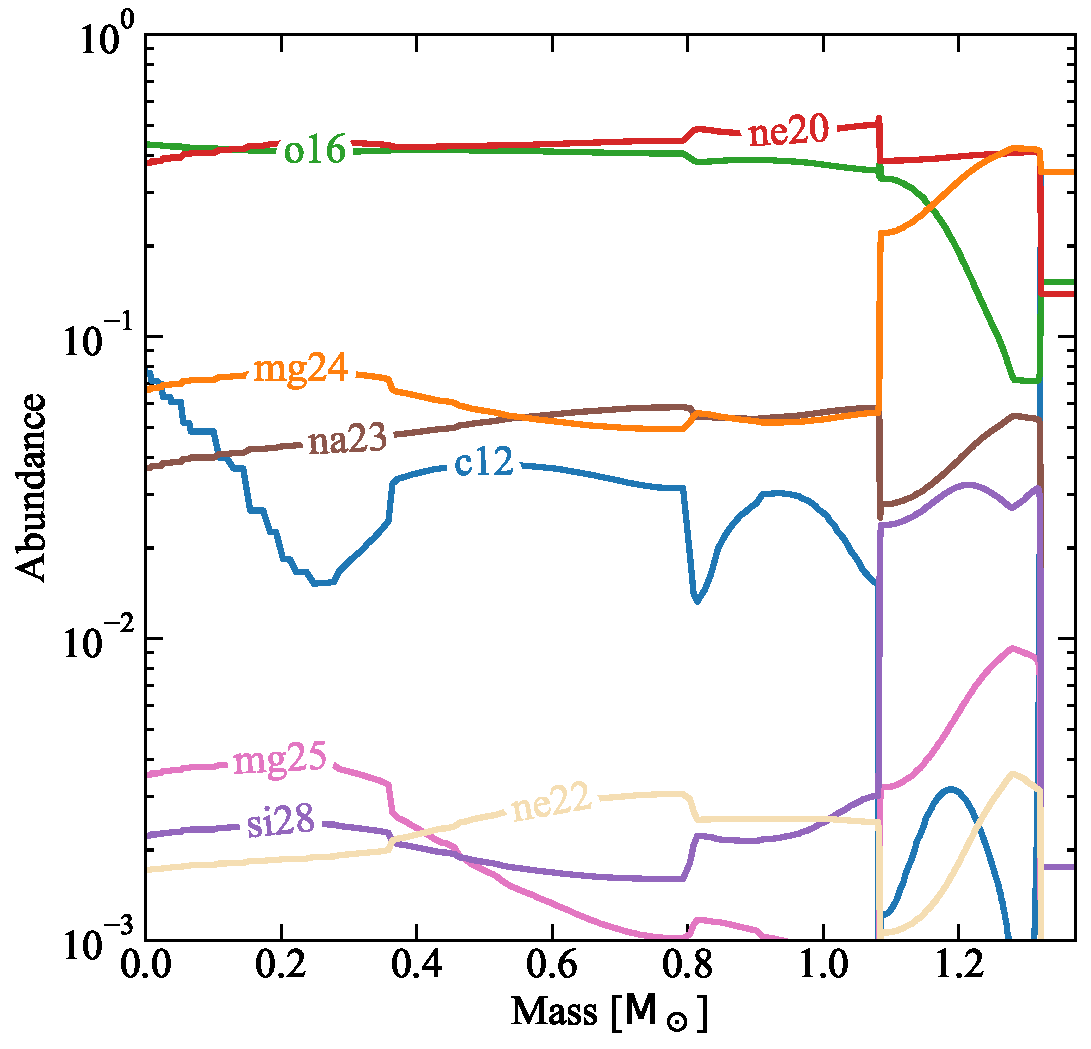
\includegraphics[height=8cm]{figures/chapter2/abundances/2p1_eta1p58_Rho9.pdf}\quad
    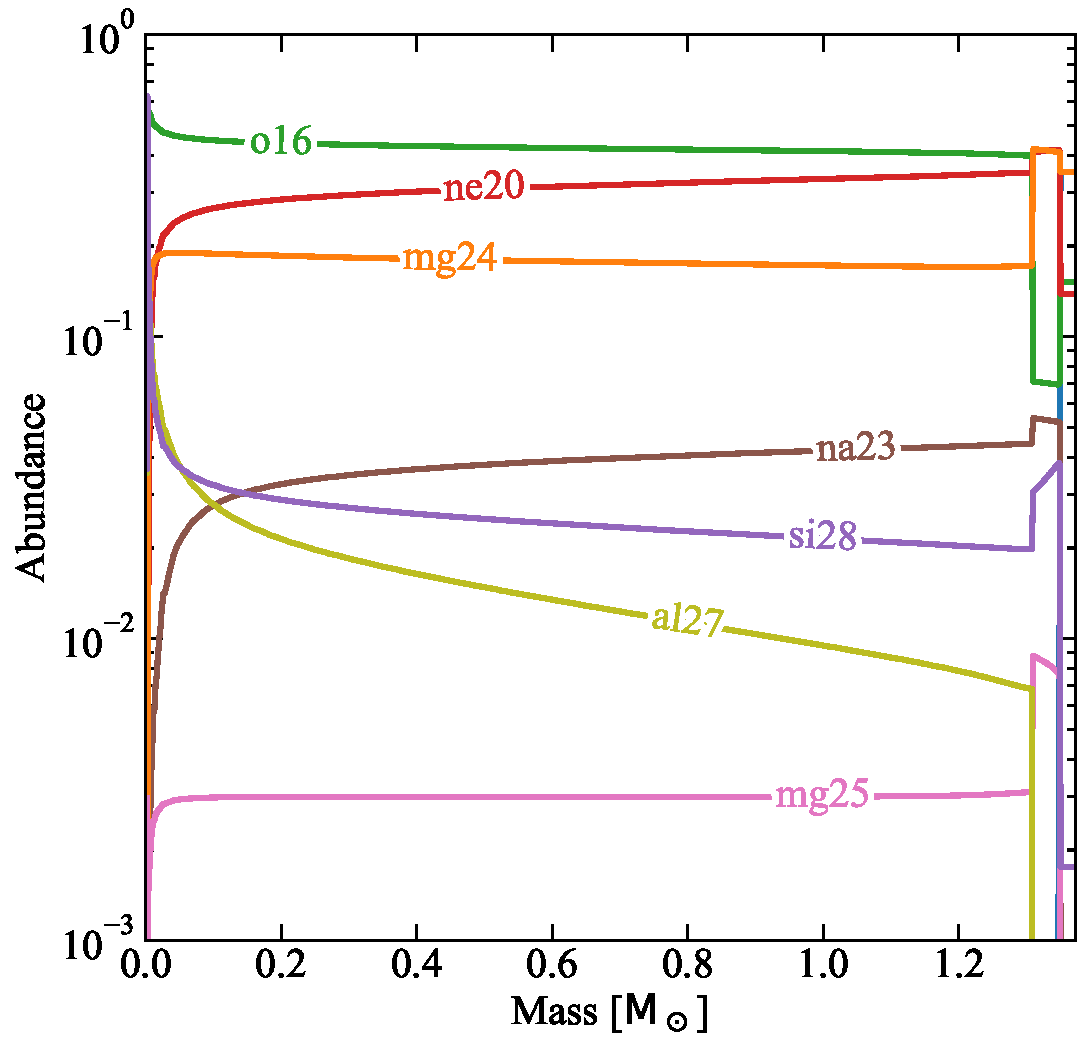
\includegraphics[height=8cm]{figures/chapter2/abundances/2p1_eta1p58_final_abun.pdf}
    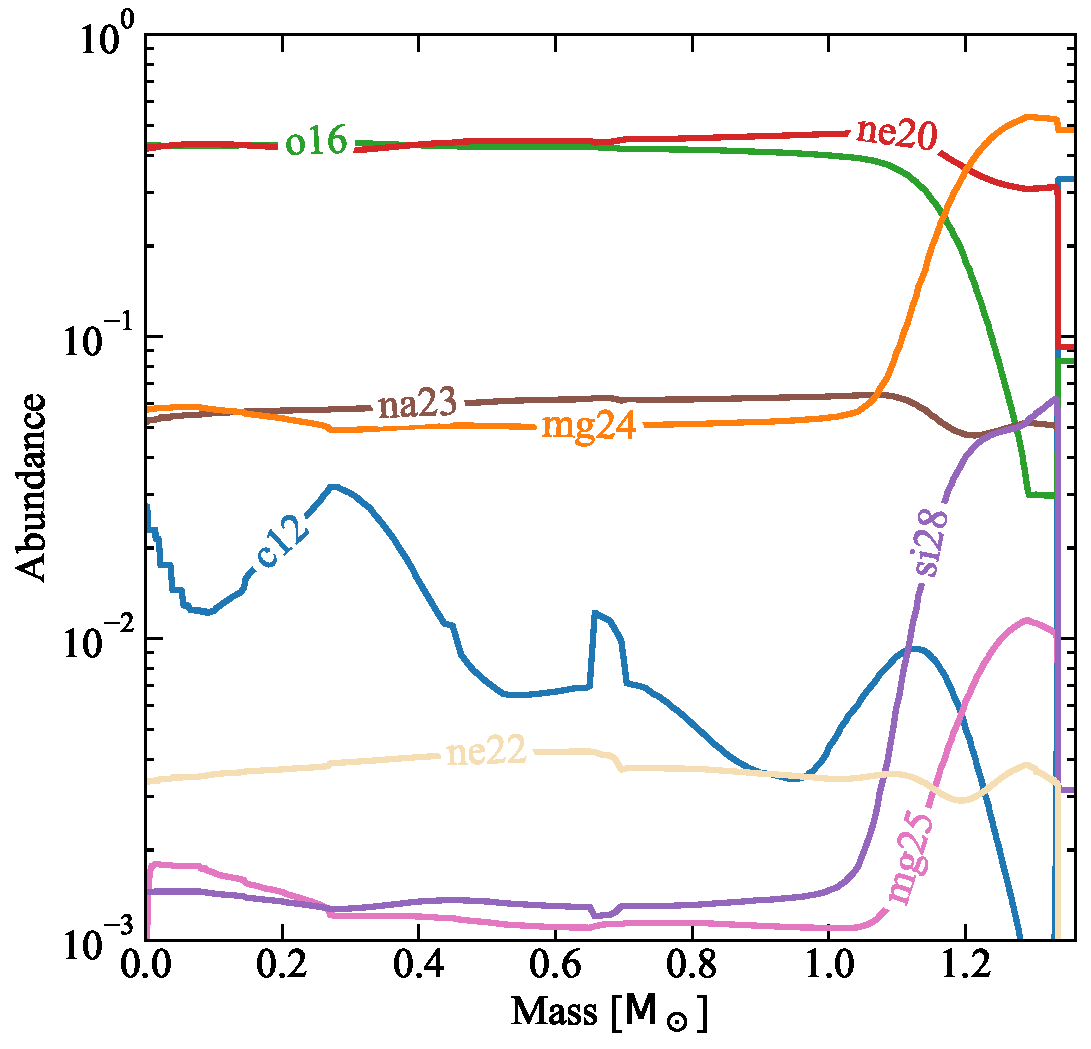
\includegraphics[height=8cm]{figures/chapter2/abundances/2p4_eta1p58_Rho9.pdf}\quad
    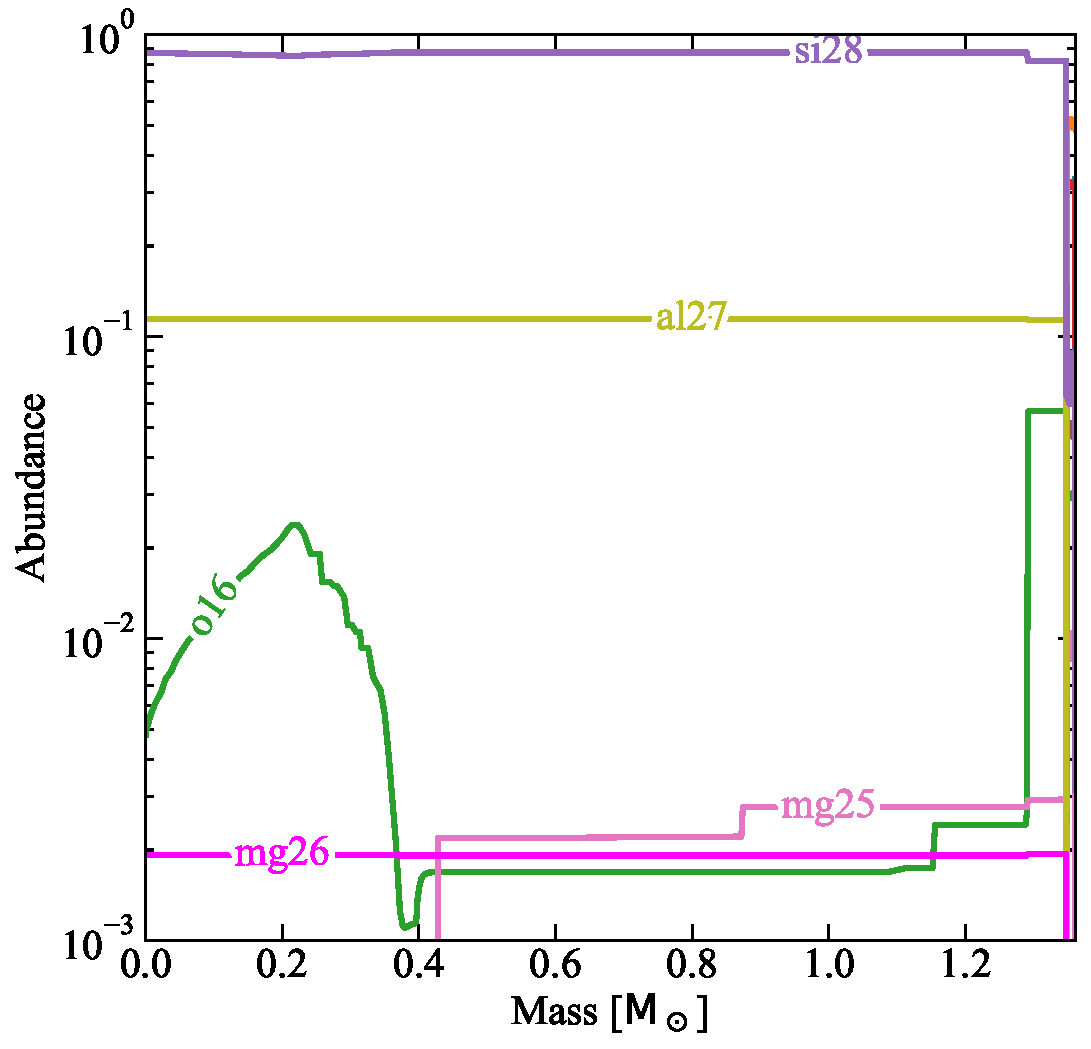
\includegraphics[height=8cm]{figures/chapter2/abundances/2p4_eta1p58_final_abun.pdf}
    \caption{Abundance profiles for two of our \seriestwo models with $2.1\msun,  Z=0.02;f_{OV}=0.0; \eta=1.6$ (top panel) and $2.4\msun,  Z=0.02;f_{OV}=0.0; \eta=1.6$ (bottom panel). On the left, the plots refer to chemical composition when $\rm \log(\rho_c / g \ cm^{-3}) \simeq 9.0$ (shortly before the Urca cooling phase). On the right, the plots refer to the final chemical composition of our models. In the case of the $2.4\msun$ model, off-center ignition of oxygen leads to the formation of a silicon core with amounts of residual oxygen distributed within the core.}
    \label{apx:fig:eta1p58}
\end{figure*}

\end{document}